\documentclass{standalone}
\usepackage{amsmath}
\newcommand{\mathup}{\mathrm}
\usepackage{sourcesanspro}
\usepackage{tikz}
\usetikzlibrary{arrows,arrows.meta,shapes,positioning,decorations.markings,angles,quotes}
\tikzset{
  % style to add an arrow in the middle of a path
  mid arrow/.style={postaction={decorate,decoration={
        markings,
        mark=at position .5 with {\arrow[#1,scale=1.5]{stealth}}
      }}},
}
\newcommand{\midarrow}{\tikz \draw[-triangle 45] (0,0) -- +(.1,0);}
\begin{document}
\sffamily
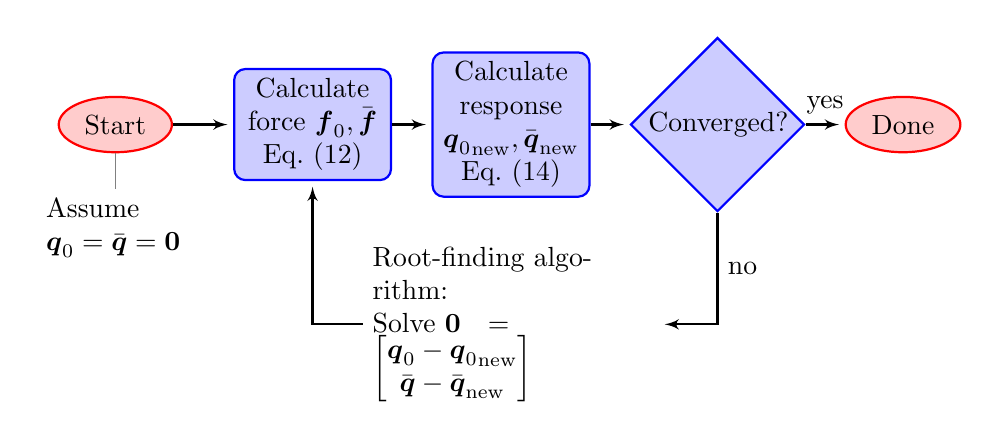
\begin{tikzpicture}
  [auto,
  decision/.style={diamond, draw=blue, thick,
    fill=blue!20, text width=5em,align=flush center,
    inner sep=1pt},
  block/.style={rectangle, draw=blue, thick, fill=blue!20,
    text width=5em,align=center, rounded corners, minimum
    height=4em},
  line/.style={draw, thick, -latex',shorten >=2pt},
  cloud/.style={draw=red, thick, ellipse,fill=red!20, minimum
    height=2em}]
  \matrix [column sep=5mm,row sep=-5mm] {
    % row 1
    \node [cloud,pin={[text width=5em]below:Assume\\$\boldsymbol{q}_0 =
      \bar{\boldsymbol{q}} = \boldsymbol{0}$}] (start){Start}; &
    % \eqref{eq:141}
    \node [block] (harmonic) {Calculate force ${\boldsymbol{f}_0}, \bar{\boldsymbol{f}}$ \\ Eq.~(12)}; &
    % \eqref{eq:142}
    \node [block] (response) {Calculate response
      ${\boldsymbol{q}_0}_{\mathup{new}}, \bar{\boldsymbol{q}}_{\mathup{new}}$ \\
      Eq.~(14)}; & \node [decision] (decide) {Converged?};
    &
    \node [cloud] (end) {Done}; \\
  };
  \node[text width=10em,node distance=5mm,below=of response] (iter)
  {Root-finding algorithm:\\ Solve $\boldsymbol{0} = \begin{bmatrix}
      \boldsymbol{q}_0 - {\boldsymbol{q}_0}_{\mathup{new}} \\
      \bar{\boldsymbol{q}} - \bar{\boldsymbol{q}}_{\mathup{new}}
    \end{bmatrix}$};
  \begin{scope}[every path/.style=line]
    \path (start) -- (harmonic); \path (harmonic) -- (response);
    \path (response) -- (decide); \path (decide) |- node [near
    start] {no} (iter); \path (iter) -| (harmonic); \path (decide)
    -- node [midway] {yes} (end);
    % \path [dashed] (system) -- (init);
    % \path [dashed] (system) |- (evaluate);
  \end{scope}
\end{tikzpicture}
\end{document}
